\documentclass{article}



\usepackage{fullpage}
\usepackage{nopageno}
\usepackage{amsmath}
\usepackage{amsfonts}
\usepackage{graphicx}
\usepackage{framed}
\usepackage{xcolor}

\definecolor{dark_red}{rgb}{0.5,0.0,0.0}
\definecolor{dark_green}{rgb}{0.0,0.5,0.0}
\definecolor{dark_blue}{rgb}{0.0,0.0,0.5}

\newcommand{\dr}[1]{\textcolor{dark_red}{#1}}
\newcommand{\dg}[1]{\textcolor{dark_green}{#1}}
\newcommand{\db}[1]{\textcolor{dark_blue}{#1}}


\begin{document}


\section*{Review}

\begin{tabular}{cc}
\parbox{0.5\textwidth}{
An arbitrary triangle will have its sides labeled \(A\), \(B\), and \(C\), and the opposite angles will be respective labeled \(\theta_A\), \(\theta_B\), and \(\theta_C\). The toolbox of equations that are used to find missing pieces of information are:
\begin{itemize}
\item \(\theta_A + \theta_B + \theta_C = 180^\circ\) ~~~~~~~~ (triangles angles add to \(180^\circ\))
\item \(\frac{A}{\sin\theta_A} = \frac{B}{\sin\theta_B} = \frac{C}{\sin\theta_C}\) ~~~~~~~~ (sine law)
\item \(A^2 = B^2 + C^2 - 2BC\cos\theta_A\) ~~~~~~~~ (cosine law)
\item \(B^2 = A^2 + C^2 - 2AC\cos\theta_B\) ~~~~~~~~ (cosine law)
\item \(C^2 = A^2 + B^2 - 2AB\cos\theta_C\) ~~~~~~~~ (cosine law)
\end{itemize}
} & \parbox{0.5\textwidth}{
\includegraphics[width = 0.5\textwidth]{general_triangle}
}
\end{tabular}

The sine law equations give:
\[A = \frac{B\sin\theta_A}{\sin\theta_B} = \frac{C\sin\theta_A}{\sin\theta_C} \quad\text{and}\quad B = \frac{A\sin\theta_B}{\sin\theta_A} = \frac{C\sin\theta_B}{\sin\theta_C} \quad\text{and}\quad C = \frac{A\sin\theta_C}{\sin\theta_A} = \frac{B\sin\theta_C}{\sin\theta_B}\]
and
\[\sin\theta_A = \frac{A\sin\theta_B}{B} = \frac{A\sin\theta_C}{C} \quad\text{and}\quad \sin\theta_B = \frac{B\sin\theta_A}{A} = \frac{B\sin\theta_C}{C} \quad\text{and}\quad \sin\theta_C = \frac{C\sin\theta_A}{A} = \frac{C\sin\theta_B}{B}\]

The cosine law equations give:
\begin{itemize}
\item \(A = \sqrt{B^2 + C^2 - 2BC\cos\theta_A} \quad\text{and}\quad \cos\theta_A = \frac{B^2 + C^2 - A^2}{2BC}\)
\item \(B = \sqrt{A^2 + C^2 - 2AC\cos\theta_B} \quad\text{and}\quad \cos\theta_B = \frac{A^2 + C^2 - B^2}{2AC}\)
\item \(C = \sqrt{A^2 + B^2 - 2AB\cos\theta_C} \quad\text{and}\quad \cos\theta_C = \frac{A^2 + B^2 - C^2}{2AB}\)
\end{itemize}

When solving triangles, the assignment of the labels of \(A\), \(B\), and \(C\) to the sides will be done arbitrarily. 



\section*{Vectors}

\begin{tabular}{cc}
\parbox{0.5\textwidth}{
A {\bf vector} is a quantity defined by ``magnitude" and ``direction". A vector is most commonly envisioned as an arrow where the length of the arrow is the magnitude, and the direction in which the arrow is pointing is the direction. Variables that represent vectors are written in boldface such as \(\mathbf{u}\), \(\mathbf{v}\), and \(\mathbf{w}\); or with a left to right arrow above the variable such as \(\vec{u}\), \(\vec{v}\), and \(\vec{w}\). 

If two vectors have the {\bf same length and direction}, then they are {\bf equal}.

The ``zero vector", denoted by \(\mathbf{0}\) or \(\vec{0}\), is a vector with a length of \(0\), and since the length is \(0\), has no direction.  

Given an arbitrary vector \(\mathbf{v}\), the magnitude/length of \(\mathbf{v}\) is denoted by \(|\mathbf{v}|\) or by \(\|\mathbf{v}\|\).
} & \parbox{0.5\textwidth}{
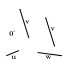
\includegraphics[width = 0.5\textwidth]{basic_vectors}
}
\end{tabular}

Quantities that do not have any direction, such as real numbers, are referred to as {\bf scalars}. The scalars used in this course will invariably be {\bf real numbers}.



\subsection*{Common vector quantities}

Below will be described some quantities that are commonly denoted using vectors.

\subsubsection*{Displacement and Position}

~~

\begin{tabular}{cc}
\parbox{0.5\textwidth}{
{\bf Displacement} is the position of one point {\bf relative} to another point. Displacement incorporates more than distance. Displacement can also be envisioned as describing a change in position. The displacement from point \(A\) to point \(B\) is a vector whose tail is on point \(A\) and whose head is on point \(B\), and is quantified by both the distance of \(B\) from \(A\), and the direction of \(B\) from \(A\). Distance is the magnitude of displacement. In the image on the right, the displacement of point \(B\) relative to point \(A\) is the vector \(\mathbf{u}\). The displacement of point \(F\) relative to point \(E\) is also \(\mathbf{u}\). 

It is important to note that displacement includes both distance and direction. In the image to the right both points \(B\) and \(C\) are located a distance of \(d\) from \(A\), but since a different direction must be used to reach \(C\) from \(A\) as opposed to reaching \(B\) from \(A\), the displacement of \(\mathbf{v}\) from \(A\) to \(C\) is not equal to \(\mathbf{u}\). Hence \(\mathbf{v} \neq \mathbf{u}\). 
} & \parbox{0.5\textwidth}{
\includegraphics[width = 0.5\textwidth]{displacement_vs_distance}
} 
\end{tabular}

\begin{tabular}{cc}
\parbox{0.5\textwidth}{
Displacement can also be used to describe position. In the image to the right, point \(A\) is chosen as the ``origin point". The positions of points \(B\), \(C\), \(D\), \(E\), and \(F\) are respectively the vectors \(\mathbf{u}\), \(\mathbf{v}\), \(\mathbf{w}\), \(\mathbf{a}\), and \(\mathbf{b}\). 
} & \parbox{0.5\textwidth}{
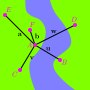
\includegraphics[width = 0.5\textwidth]{position}
}
\end{tabular}



\subsubsection*{Velocity}

~~

\begin{tabular}{cc}
\parbox{0.5\textwidth}{
{\bf Velocity} quantifies the rate of change in an object's position with respect to time. Speed on the other hand, merely quantifies the rate at which the total distance traveled changes with respect to time. Given an arbitrary velocity vector \(\mathbf{v}\), the magnitude \(\|\mathbf{v}\|\) is the object's speed, and the direction of \(\mathbf{v}\) is the direction in which the object is moving. In the image to the right, objects \(A\), \(B\), and \(C\) have the respective velocities \(\mathbf{v}_1\), \(\mathbf{v}_2\), and \(\mathbf{v}_3\), and the respective speeds of \(u_1 = \|\mathbf{v}_1\|\), \(u_2 = \|\mathbf{v}_2\|\), and \(u_3 = \|\mathbf{v}_3\|\).
} & \parbox{0.5\textwidth}{
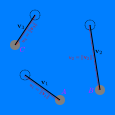
\includegraphics[width = 0.5\textwidth]{velocity}
} 
\end{tabular}





\section*{Vector operations}

\subsection*{Vector addition}

The addition of two vectors \(\mathbf{u}\) and \(\mathbf{v}\) is performed as follows: Envision both \(\mathbf{u}\) and \(\mathbf{v}\) as arrows. The ``head-to-tail" rule for addition requires that vector \(\mathbf{v}\) be translated through space without any rotation so that its ``tail" connects to the``head" of vector \(\mathbf{u}\). The sum \(\mathbf{u} + \mathbf{v}\) (referred to as the {\bf resultant vector}) is now a straight arrow whose tail is the tail of \(\mathbf{u}\), and whose head is the head of \(\mathbf{v}\). Vector addition is demonstrated in the images below. 

In the image on the left, the commutative property of vector addition is shown via a parallelogram. Connecting the tail of \(\mathbf{v}\) to the head of \(\mathbf{u}\) results in the same sum as connecting the tail of \(\mathbf{u}\) to the head of \(\mathbf{v}\). Hence \(\mathbf{u} + \mathbf{v} = \mathbf{v} + \mathbf{u}\). 

In the image on the right, the associative property of vector addition is shown. Vectors \(\mathbf{u}\), \(\mathbf{v}\), and \(\mathbf{w}\) are chained together to form the sum \(\mathbf{u} + \mathbf{v} + \mathbf{w}\) by linking the head of \(\mathbf{u}\) to the tail of \(\mathbf{v}\) and linking the head of \(\mathbf{v}\) to the tail of \(\mathbf{w}\). Whether the link between the head of \(\mathbf{u}\) and the tail of \(\mathbf{v}\) is established first, or the link between the head of \(\mathbf{v}\) and the tail of \(\mathbf{w}\) is established first, the sum is the same. Hence the associative property.

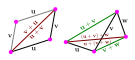
\includegraphics[width = \textwidth]{vector_addition}


\subsection*{Scalar multiplication}

While there exist multiplication operators for multiplying together two vectors, the most common form of multiplication is the multiplication of a vector and a scalar (real number).

The multiplication of vector \(\mathbf{v}\) and scalar \(c\) (\(c\) is areal number) to get \(c\mathbf{v}\), which is also equal to the expression \(\mathbf{v}c\), is to add \(c\) copies of \(\mathbf{v}\) together. If \(c\) is a natural number \(n\), then:
\[n\mathbf{v} = \underbrace{\mathbf{v} + \mathbf{v} + \cdots + \mathbf{v}}_n\]
When \(c\) is an arbitrary real number, then adding \(c\) copies of \(\mathbf{v}\) together to get \(c\mathbf{v}\) (\(= \mathbf{v}c\)) is performed as follows. Increase the magnitude of \(\mathbf{v}\) by a factor of \(|c|\) while keeping the direction the same. If \(c < 0\), then reverse the direction. Given an arbitrary vector \(\mathbf{v}\), the negative of \(\mathbf{v}\), denoted by \(-\mathbf{v}\), has the same magnitude as \(\mathbf{v}\) but the direction is reversed. The vector difference \(\mathbf{u} - \mathbf{v}\) is the addition of \(-\mathbf{v}\) to \(\mathbf{u}\): 
\[\mathbf{u} - \mathbf{v} = \mathbf{u} + (-\mathbf{v})\]
When vector \(\mathbf{v}\) is divided by the scalar \(c\), vector \(\mathbf{v}\) is being multiplied by \(\frac{1}{c}\).
\[\frac{\mathbf{v}}{c} = \frac{1}{c} \cdot \mathbf{v}\]

Below are given examples of scalar multiplication using the vector \(\mathbf{v}\) on the left. Second from the left is \(2\mathbf{v}\). Third from the left is \(0\mathbf{v}\) is which is the zero vector \(\mathbf{0}\). Fourth from the left is \(-\mathbf{v} = (-1)\mathbf{v}\) which is \(\mathbf{v}\) with the direction reversed. Second from the right is \(1.5\mathbf{v}\). On the right is \(-2\mathbf{v}\).

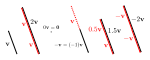
\includegraphics[width = \textwidth]{scalar_multiplication}

Below are shown the distributive laws for scalar multiplication. On the left is shown \((c + k)\mathbf{v} = c\mathbf{v} + k\mathbf{v}\). On the right is shown \(c(\mathbf{u} + \mathbf{v}) = c\mathbf{u} + c\mathbf{v}\).

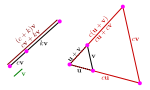
\includegraphics[width = \textwidth]{distributive_laws}

Given a velocity of \(\mathbf{v}\), and a time of \(\Delta t\), the total displacement covered in time \(\Delta t\) is \(\Delta t \cdot \mathbf{v}\).



\subsection*{Examples}

\textbf{Hiking trip:}

\begin{tabular}{cc}
\parbox{0.5\textwidth}{
Consider a hiking trip that consists of two sections. The first leg is a displacement \(\mathbf{r}_1\) that is a distance of \(d_1 = 5\text{km}\) in a direction of \(\theta_1 = 10^\circ\) south of east. The second leg is a displacement \(\mathbf{r}_2\) that is a distance of \(d_2 = 10\text{km}\) in a direction of \(\theta_2 = 5^\circ\) west of north. The total displacement from the starting point to the finishing point is \(\mathbf{r}_t = \mathbf{r}_1 + \mathbf{r}_2\). The total displacement \(\mathbf{r}_t\) has the length \(d_t\) and has a direction of \(\theta_t\) east of north. To find the resultant displacement \(\mathbf{r}_t\), the triangle formed by the sum \(\mathbf{r}_t = \mathbf{r}_1 + \mathbf{r}_2\) has the following information known: \(A = d_1 = 5\text{km}\), \(B = d_2 = 10\text{km}\), and \(\theta_C = 90^\circ - \theta_1 - \theta_2 = 75^\circ\). Via the cosine law, \(d_t = C = \sqrt{A^2 + B^2 - 2AB\cos\theta_C} \approx 9.95581\text{km}\). With \(C\) now known, \(\theta_B = \cos^{-1}\left(\frac{A^2 + C^2 - B^2}{2AC}\right) \approx 75.9805^\circ\). Angle \(\theta_B\) is also \(\theta_B = 90^\circ + \theta_1 - \theta_t\) so \(\theta_t = 90^\circ + \theta_1 - \theta_B \approx 24.0195^\circ\). Therefore the total displacement \(\mathbf{r}_t\) is \(d_t \approx 9.95581\text{km}\) in the direction of \(\theta_t \approx 24.0195^\circ\) east of north.
} & \parbox{0.5\textwidth}{
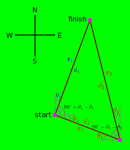
\includegraphics[width = 0.5\textwidth]{hiking_trip}
}
\end{tabular}



\vspace{5mm}

\textbf{Wind and flight:}

\begin{tabular}{cc}
\parbox{0.5\textwidth}{
The image on the right shows scenario where the wind is blowing with speed \(u_w = 500\text{km/h}\) at an angle of \(\phi_w = 25^\circ\) east of south. These two quantities together define the wind's velocity of \(\mathbf{v}_w\). A plane with air speed \(u_p = 800\text{km/h}\) is oriented at an angle of \(\phi_p = 35^\circ\) east of north. These two quantities together define the plane's air velocity of \(\mathbf{v}_p\). The plane's velocity is being measured against the air and not the ground, and the air is moving. In time \(\Delta t\), the air has shoved the plane a displacement of \(\mathbf{v}_w \cdot \Delta t\) against the ground. Against the air, the plane has traveled a displacement of \(\mathbf{v}_p \cdot \Delta t\). Against the ground, the plane has traveled a displacement of \(\mathbf{v}_t \cdot \Delta t\), where \(\mathbf{v}_t\) is the resultant velocity. This displacement against the ground is the sum of the air's displacement against the ground and the plane's displacement against the air: \(\mathbf{v}_t \cdot \Delta t = \mathbf{v}_w \cdot \Delta t + \mathbf{v}_p \cdot \Delta t\) which is equivalent to \(\mathbf{v}_t = \mathbf{v}_w + \mathbf{v}_p\). The resultant ground speed of \(u_t = \|\mathbf{v}_t\|\) and direction \(\phi_t\) east of north are the sought after quantities. These two quantities together define the plane's ground velocity of \(\mathbf{v}_t\).    
} & \parbox{0.5\textwidth}{
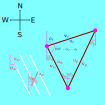
\includegraphics[width = 0.5\textwidth]{wind_currents}
}
\end{tabular}

To find the ground velocity \(\mathbf{v}_t\), the triangle formed by the sum \(\mathbf{v}_t = \mathbf{v}_w + \mathbf{v}_p\) has the following information known: \(A = u_w = 500\text{km/h}\), \(B = u_p = 800\text{km/h}\), and \(\theta_C = \phi_w + \phi_p = 60^\circ\). Via the cosine law, \(u_t = C = \sqrt{A^2 + B^2 - 2AB\cos\theta_C} = 700\text{km/h}\). With \(C\) now known, \(\theta_B = \cos^{-1}\left(\frac{A^2 + C^2 - B^2}{2AC}\right) \approx 81.7868^\circ\). Angle \(\theta_B\) is also \(\theta_B = 180^\circ - \phi_w - \phi_t\) so \(\phi_t = 180^\circ - \phi_w - \theta_B \approx 73.2132^\circ\). Therefore the ground velocity is \(u_t = 700\text{km/h}\) in the direction of \(\phi_t \approx 73.2132^\circ\) east of north.



\vspace{5mm}

\textbf{Tension example:}

\begin{tabular}{cc}
\parbox{0.4\textwidth}{
If the image to the right, a mass with a weight of \(F_g = 1000\text{N}\) is suspended by two cables. The left and right cables make respective angles of \(\theta_1 = 27^\circ\) and \(\theta_2 = 52^\circ\) to the vertical direction. The tensions of \(T_1\) and \(T_2\) is the left and right cables are the quantities that are sought. There are 3 forces acting on the junction connecting the cables. There are the tension forces \(\mathbf{G}_1\) and \(\mathbf{G}_2\) from the left and right cables respectively. There is the gravitational force of \(\mathbf{G}_3\). For equilibrium, all 3 of these forces must add to \(\mathbf{0}\): It must be the case that \(\mathbf{G}_1 + \mathbf{G}_2 + \mathbf{G}_3 = \mathbf{0}\). The magnitudes of \(\mathbf{G}_1\), \(\mathbf{G}_2\), and \(\mathbf{G}_3\) are respectively \(\|\mathbf{G}_1\| = T_1\), \(\|\mathbf{G}_2\| = T_2\), and \(\|\mathbf{G}_3\| = F_g\). 
} & \parbox{0.6\textwidth}{
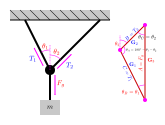
\includegraphics[width = 0.6\textwidth]{hanging_mass}
}
\end{tabular}

In the triangle formed by the sum \(\mathbf{G}_1 + \mathbf{G}_2 + \mathbf{G}_3 = \mathbf{0}\), the known quantities are: \(A = F_g = 1000\text{N}\), \(\theta_B = \theta_1 = 27^\circ\), and \(\theta_C = \theta_2 = 52^\circ\). Using the fact that the angles in a triangle sum to \(180^\circ\), we get \(\theta_A = 180^\circ - \theta_B - \theta_C = 180^\circ - \theta_1 - \theta_2 = 180^\circ - 27^\circ - 52^\circ = 101^\circ\). The sine law is, 
\[\frac{A}{\sin\theta_A} = \frac{B}{\sin\theta_B} = \frac{C}{\sin\theta_C} \iff \frac{1000\text{N}}{\sin 101^\circ} = \frac{B}{\sin 27^\circ} = \frac{C}{\sin 52^\circ}\]
so \(B = \frac{(1000\text{N})\sin 27^\circ}{\sin 101^\circ} \approx 462.488\text{N}\) and \(C = \frac{(1000\text{N})\sin 52^\circ}{\sin 101^\circ} \approx 802.760\text{N}\). Therefore \(T_1 = C \approx 802.760\text{N}\) and \(T_2 = B \approx 462.488\text{N}\).




\section*{Vectors in Component Form}


\begin{tabular}{cc}
\parbox{0.5\textwidth}{
Establishing an \(xy\) Cartesian coordinate system, an arbitrary vector can be expressed as the sum of a component that is parallel to the x-axis, and a component that is parallel to the y-axis. Given a vector \(\mathbf{v}\), let \(v_x\) denote the x-coordinate difference between the head and tail, and let \(v_y\) denote the y-coordinate difference between the head and tail. \(\mathbf{v}\) will then be denoted via: \(\mathbf{v} = \langle v_x, v_y \rangle\). \(\mathbf{i}\) is a vector of length \(1\) (unit vector) that points in the direction of the positive \(x\)-axis. \(\mathbf{j}\) is a vector of length \(1\) (unit vector) that points in the direction of the positive \(y\)-axis. Together, \(\mathbf{i}\) and \(\mathbf{j}\) form the set of ``elementary basis vectors". The horizontal component of \(\mathbf{v}\) is \(v_x\mathbf{i}\), and the vertical component is \(v_y\mathbf{j}\), so \(\mathbf{v} = v_x\mathbf{i} + v_y\mathbf{j}\). The expression \(v_x\mathbf{i} + v_y\mathbf{j}\) is a ``linear combination" of the vectors \(\mathbf{i}\) and \(\mathbf{j}\).
} & \parbox{0.5\textwidth}{
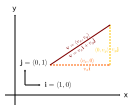
\includegraphics[width = 0.5\textwidth]{component_form}
}
\end{tabular}

\begin{tabular}{cc}
\parbox{0.5\textwidth}{
The image on the right shows example vectors in component form. Copies of \(\mathbf{i}\) and \(\mathbf{j}\) are added together to form the shown vectors.
} & \parbox{0.5\textwidth}{
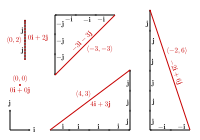
\includegraphics[width = 0.5\textwidth]{component_vector_examples}
}
\end{tabular}

Below is described the math associated with vectors in component form.
\begin{itemize}
\item The addition of two vectors in component form is: \(\langle u_x, u_y \rangle + \langle v_x, v_y \rangle = \langle u_x + v_x, u_y + v_y \rangle\) \\
Proof:
\begin{align*}
\langle u_x, u_y \rangle + \langle v_x, v_y \rangle = & (u_x\mathbf{i} + u_y\mathbf{j}) + (v_x\mathbf{i} + v_y\mathbf{j}) 
= (u_x\mathbf{i} + v_x\mathbf{i}) + (u_y\mathbf{j} + v_y\mathbf{j}) \\
= & (u_x + v_x)\mathbf{i} + (u_y + v_y)\mathbf{j} 
= \langle u_x + v_x , u_y + v_y \rangle 
\end{align*}
\item The multiplication of a vector in component form by a scalar is: \(c\langle v_x, v_y \rangle = \langle c v_x, c v_y \rangle\) \\
Proof:
\begin{align*}
c\langle v_x, v_y \rangle =  & c(v_x\mathbf{i} + v_y\mathbf{j})
= cv_x\mathbf{i} + cv_y\mathbf{j}
= \langle cv_x, cv_y \rangle
\end{align*}
\item The magnitude (length) of a vector in component form is: \(\|\langle v_x, v_y \rangle\| = \sqrt{v_x^2 + v_y^2}\) \\
Proof: \\
The Pythagorean theorem gives: \(\|\langle v_x, v_y \rangle\|^2 = v_x^2 + v_y^2\) so \(\|\langle v_x, v_y \rangle\| = \sqrt{v_x^2 + v_y^2}\)  
\end{itemize}



\subsection*{Component vector addition}

\begin{tabular}{cc}
\parbox{0.5\textwidth}{
A major benefit of vectors expressed using component form is that the addition and scalar multiplication of vectors is a trivial matter. Consider two vectors \(\mathbf{u} = \langle u_x, u_y \rangle\) and \(\mathbf{v} = \langle v_x, v_y \rangle\). Adding vectors \(\mathbf{u}\) and \(\mathbf{v}\), as seen in the image on the right, involves adding the horizontal components of \(\mathbf{u}\) and \(\mathbf{v}\) to get the horizontal component of \(\mathbf{u} + \mathbf{v}\); and adding the vertical components of \(\mathbf{u}\) and \(\mathbf{v}\) to get the vertical component of \(\mathbf{u} + \mathbf{v}\). The horizontal component of \(\mathbf{u} + \mathbf{v}\) is \(u_x\mathbf{i} + v_x\mathbf{i} = (u_x + v_x)\mathbf{i}\). The vertical component of \(\mathbf{u} + \mathbf{v}\) is \(u_y\mathbf{j} + v_y\mathbf{j} = (u_y + v_y)\mathbf{j}\). Therefore:
\[\mathbf{u} + \mathbf{v} = \langle u_x + v_x, u_y + v_y \rangle\]
Vectors are added by simply adding together their corresponding horizontal and vertical components.
} & \parbox{0.5\textwidth}{
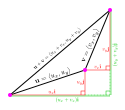
\includegraphics[width = 0.5\textwidth]{component_vector_addition}
}
\end{tabular}

\textbf{Examples:}
\begin{itemize}
\item \(\langle 11, 9 \rangle + \langle -5, -7 \rangle = \langle 11 - 5, 9 - 7 \rangle = \langle 6, 2 \rangle\)
\item \(\langle 34, -24 \rangle + \langle 23, 41 \rangle = \langle 34 + 23, -24 + 41 \rangle = \langle 57, 17 \rangle\)
\item \(\langle 2, -24 \rangle + \langle 18, 21 \rangle = \langle 2 + 18, -24 + 21 \rangle = \langle 20, -3 \rangle\)
\end{itemize}


\subsection*{Component vector negatives}

\begin{tabular}{cc}
\parbox{0.5\textwidth}{
The negative of a vector \(\mathbf{v} = \langle v_x, v_y \rangle\) is determined by simply reversing the direction of \(\mathbf{v}\). In terms of components, the sign of each component is flipped:
\[-\mathbf{v} = \langle -v_x, -v_y \rangle\]
When a vector \(\mathbf{v}\) is subtracted from a vector \(\mathbf{u}\), what is happening is that the negative of \(\mathbf{v}\) is being added to \(\mathbf{u}\): 
\[\mathbf{u} - \mathbf{v} = \mathbf{u} + (-\mathbf{v})\]
} & \parbox{0.5\textwidth}{
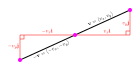
\includegraphics[width = 0.5\textwidth]{component_vector_negative}
}
\end{tabular}
\[\langle u_x, u_y \rangle - \langle v_x, v_y \rangle = \langle u_x, u_y \rangle + \langle -v_x, -v_y \rangle = \langle u_x - v_x, u_y - v_y \rangle\]


\subsection*{Component vector scalar multiplication}

Consider an arbitrary vector \(\mathbf{v} = \langle v_x, v_y \rangle\). For an arbitrary natural number \(n \in \{1, 2, 3, ...\}\), adding \(n\) copies of \(\mathbf{v}\) together gives \(n\mathbf{v}\):
\begin{align*}
n\mathbf{v} = & \underbrace{\mathbf{v} + \mathbf{v} + \cdots + \mathbf{v}}_n 
= \underbrace{\langle v_x, v_y \rangle + \langle v_x, v_y \rangle + \cdots + \langle v_x, v_y \rangle}_n 
= \left\langle \underbrace{v_x + v_x + \cdots + v_x}_n, \underbrace{v_y + v_y + \cdots + v_y}_n \right\rangle \\  
= & \langle n v_x, n v_y \rangle
\end{align*}
Therefore:
\[n\mathbf{v} = \langle n v_x, n v_y \rangle\]

Generalizing the natural number \(n\) to a real number \(c \in \mathbb{R}\) gives the general formula scalar multiplication:
\[c\mathbf{v} = \langle c v_x, c v_y \rangle\]
In essence, multiplication by a scalar \(c\) simply involves the multiplication of each component by \(c\). \\

Dividing a vector \(\mathbf{v} = \langle v_x, v_y \rangle\) by a scalar \(c\) is performed by dividing each component by \(c\). This is equivalent to multiplying the vector by \(\frac{1}{c}\):
\[\frac{\mathbf{v}}{c} = \frac{1}{c} \cdot \mathbf{v} = \langle \frac{v_x}{c}, \frac{v_y}{c} \rangle\]

\textbf{Examples:}
\begin{itemize}
\item \(3\langle -1, 5 \rangle = \langle 3 \cdot (-1), 3 \cdot 5 \rangle = \langle -3, 15 \rangle\)
\item \(-2\langle 4, 7 \rangle = \langle (-2) \cdot 4, (-2) \cdot 7 \rangle = \langle -8, -14 \rangle\)
\item \(5\langle 0.2, -1.2 \rangle = \langle 5 \cdot (0.2), 5 \cdot (-1.2) \rangle = \langle 1, -6 \rangle\)
\item \(\frac{\langle 12, -8 \rangle}{4} = \langle \frac{12}{4} , \frac{-8}{4} \rangle = \langle 3, -2 \rangle\)
\end{itemize}


\subsection*{Component vector magnitude}

\begin{tabular}{cc}
\parbox{0.5\textwidth}{
Consider an arbitrary vector \(\mathbf{v} = \langle v_x, v_y \rangle\). Through use of the Pythagorean theorem, the length (or magnitude) of \(\mathbf{v}\), denoted by \(\|\mathbf{v}\|\), satisfies \(\|\mathbf{v}\|^2 = |v_x|^2 + |v_y|^2\). Therefore:
\[\|\mathbf{v}\| = \sqrt{v_x^2 + v_y^2}\]
} & \parbox{0.5\textwidth}{
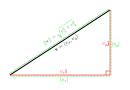
\includegraphics[width = 0.5\textwidth]{component_vector_magnitude}
}
\end{tabular}

\textbf{Examples:}
\begin{itemize}
\item \(\|\langle -3, 4 \rangle\| = \sqrt{(-3)^2 + 4^2} = \sqrt{9 + 16} = \sqrt{25} = 5\)
\item \(\|\langle 12, -5 \rangle\| = \sqrt{12^2 + (-5)^2} = \sqrt{144 + 25} = \sqrt{169} = 13\)
\item \(\|\langle -3, -1 \rangle\| = \sqrt{(-3)^2 + (-1)^2} = \sqrt{9 + 1} = \sqrt{10} \approx 3.16228\)
\end{itemize}


\subsection*{Putting it all together}

\begin{itemize}
\item \(6\langle 2, -3 \rangle - \langle -5, 7 \rangle = \langle 12, -18 \rangle + \langle 5, -7 \rangle = \langle 17, -25 \rangle\)
\item \(\|\langle 3, 2 \rangle + 2\langle 1.5, -0.5 \rangle\| = \|\langle 3, 2 \rangle + \langle 3, -1 \rangle\| = \|\langle 6, 1 \rangle\| = \sqrt{6^2 + 1^2} = \sqrt{37} \approx 6.08276\)
\item \(\frac{\langle 6, -4 \rangle}{2} - 3\langle 0, 5 \rangle = \frac{1}{2}\langle 6, -4 \rangle + \langle 0, -15 \rangle = \langle 3, -2 \rangle + \langle 0, -15 \rangle = \langle 3, -17 \rangle\)
\item \(\langle 5, -8 \rangle + \langle -2, 6 \rangle = \langle (5) + (-2) , (-8) + (6) \rangle = \langle 3 , -2 \rangle\)
\item \(3 \langle -2, 4 \rangle = \langle (3)(-2), (3)(4) \rangle = \langle -6, 12 \rangle\)
\item \(-7 \langle 5, 2 \rangle + 5 \langle 2, 3 \rangle = \langle -35, -14 \rangle + \langle 10, 15 \rangle = \langle -25, 1 \rangle\)
\item \(\|\langle 6, 8 \rangle\| = \sqrt{6^2 + 8^2} = \sqrt{36 + 64} = \sqrt{100} = 10\)
\end{itemize}


\subsection*{Deriving the horizontal and vertical components from the length and direction}

There are two ways of quantifying vectors. The first approach is to quantify a vector using its length and direction. The second approach is to quantify a vector using its horizontal and vertical components. In many circumstances it is necessary to convert between the two forms.


Below, the process of deriving the components of a vector when given its length and direction, is shown. There are 8 possible cases. It is important to know how to derive these cases instead of memorizing them. When a vector has:
\begin{itemize}
\item A length of \(r_1\), and an angle of \(\theta_1\) above the positive x-axis: \(\mathbf{v}_1 = \langle r_1\cos\theta_1, r_1\sin\theta_1 \rangle\)
\item A length of \(r_1\), and an angle of \(\phi_1\) right of the positive y-axis: \(\mathbf{v}_1 = \langle r_1\sin\phi_1, r_1\cos\phi_1 \rangle\)
\item A length of \(r_2\), and an angle of \(\theta_2\) left of the positive y-axis: \(\mathbf{v}_2 = \langle -r_2\sin\theta_2, r_2\cos\theta_2 \rangle\)
\item A length of \(r_2\), and an angle of \(\phi_2\) above the negative x-axis: \(\mathbf{v}_2 = \langle -r_2\cos\phi_2, r_2\sin\phi_2 \rangle\)
\item A length of \(r_3\), and an angle of \(\theta_3\) below the negative x-axis: \(\mathbf{v}_3 = \langle -r_3\cos\theta_3, -r_3\sin\theta_3 \rangle\)
\item A length of \(r_3\), and an angle of \(\phi_3\) left of the negative y-axis: \(\mathbf{v}_3 = \langle -r_3\sin\phi_3, -r_3\cos\phi_3 \rangle\)
\item A length of \(r_4\), and an angle of \(\theta_4\) right of the negative y-axis: \(\mathbf{v}_4 = \langle r_4\sin\theta_4, -r_4\cos\theta_4 \rangle\)
\item A length of \(r_4\), and an angle of \(\phi_4\) below the positive x-axis: \(\mathbf{v}_4 = \langle r_4\cos\phi_4, -r_4\sin\phi_4 \rangle\)
\end{itemize}
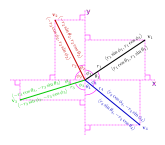
\includegraphics[width = \textwidth]{polar_vector_to_cartesian_vector}

\textbf{Examples:}
\begin{itemize}
%%%%%%%%%%%%%
\item Given a vector \(\mathbf{v}\) where \(\|\mathbf{v}\| = 5\) and the direction is \(\theta = 30^\circ\) above the positive x-axis, then \(\mathbf{v} = \langle 5\cos 30^\circ, 5\sin 30^\circ \rangle \approx \langle 4.33013, 2.50000 \rangle\)
%%%%%%%%%%%%%
\item Given a vector \(\mathbf{v}\) where \(\|\mathbf{v}\| = 6\) and the direction is \(\theta = 20^\circ\) left of the negative y-axis, then \(\mathbf{v} = \langle -6\sin 20^\circ, -6\cos 20^\circ \rangle \approx \langle -2.05212, -5.63816 \rangle\)
%%%%%%%%%%%%%
\item Given a vector \(\mathbf{v}\) where \(\|\mathbf{v}\| = 7\) and the direction is \(\theta = 25^\circ\) beneath the positive x-axis, then \(\mathbf{v} = \langle 7\cos 25^\circ, -7\sin 25^\circ \rangle \approx \langle 6.34415, -2.95833 \rangle\)
%%%%%%%%%%%%%
\item Given a vector \(\mathbf{v}\) where \(\|\mathbf{v}\| = 8\) and the direction is \(\theta = 53^\circ\) left of the positive y-axis, then \(\mathbf{v} = \langle -8\sin 53^\circ, 8\cos 53^\circ \rangle \approx \langle -6.38908, 4.81452 \rangle\)
\end{itemize}



\subsection*{Deriving the length and direction from the horizontal and vertical components}

Below, the process of deriving the length and direction of a vector when given its components, is shown. Given a vector \(\mathbf{v} = \langle x, y \rangle\), the length of \(\mathbf{v}\) is always \(\|\mathbf{v}\| = \sqrt{x^2 + y^2}\). It is important to know how to derive these cases instead of memorizing them.
\begin{itemize}
\item When \(x \geq 0\) and \(y \geq 0\), the angle above the positive x-axis is \(\tan^{-1}(|y|/|x|)\), and the angle to the right of the positive y-axis is \(\tan^{-1}(|x|/|y|)\).
\item When \(x \leq 0\) and \(y \geq 0\), the angle to the left of the positive y-axis is \(\tan^{-1}(|x|/|y|)\), and the angle above the negative x-axis is \(\tan^{-1}(|y|/|x|)\).
\item When \(x \leq 0\) and \(y \leq 0\), the angle below the negative x-axis is \(\tan^{-1}(|y|/|x|)\), and the angle to the left of the negative y-axis is \(\tan^{-1}(|x|/|y|)\).
\item When \(x \geq 0\) and \(y \leq 0\), the angle to the right of the negative y-axis is \(\tan^{-1}(|x|/|y|)\), and the angle below the positive x-axis is \(\tan^{-1}(|y|/|x|)\).
\end{itemize}
In general, the angle measured against the \(x\)-axis, positive or negative, above or below, is \(\tan^{-1}(|y|/|x|)\), and the angle measured against the \(y\)-axis, positive or negative, right or left, is \(\tan^{-1}(|x|/|y|)\).

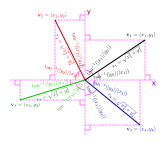
\includegraphics[width = \textwidth]{cartesian_vector_to_polar_vector}

\textbf{Examples:}
\begin{itemize}
%%%%%%%%%%%%%
\item Given the vector \(\mathbf{v} = \langle -2, 8 \rangle\), then the length is \(\|\mathbf{v}\| = \sqrt{(-2)^2 + 8^2} = \sqrt{4 + 64} = \sqrt{68} \approx 8.24621\), and the direction can be quantified as either \(\theta = \tan^{-1}(2/8) \approx 14.0362^\circ\) left of the positive y-axis, or \(\theta = \tan^{-1}(8/2) \approx 75.9638^\circ\) above the negative x-axis.
%%%%%%%%%%%%%
\item Given the vector \(\mathbf{v} = \langle -3, -5 \rangle\), then the length is \(\|\mathbf{v}\| = \sqrt{(-3)^2 + (-5)^2} = \sqrt{9 + 25} = \sqrt{34} \approx 5.83095\), and the direction can be quantified as either \(\theta = \tan^{-1}(5/3) \approx 59.0362^\circ\) below the negative x-axis, or \(\theta = \tan^{-1}(3/5) \approx 30.9638^\circ\) left of the negative y-axis.
%%%%%%%%%%%%%
\item Given the vector \(\mathbf{v} = \langle 6, 1 \rangle\), then the length is \(\|\mathbf{v}\| = \sqrt{6^2 + 1^2} = \sqrt{36 + 1} = \sqrt{37} \approx 6.08276\), and the direction can be quantified as either \(\theta = \tan^{-1}(1/6) \approx 9.46232^\circ\) above the positive x-axis, or \(\theta = \tan^{-1}(6/1) \approx 80.5377^\circ\) right of the positive y-axis.
%%%%%%%%%%%%%
\item Given the vector \(\mathbf{v} = \langle 3, -7 \rangle\), then the length is \(\|\mathbf{v}\| = \sqrt{3^2 + (-7)^2} = \sqrt{9 + 49} = \sqrt{58} \approx 7.61577\), and the direction can be quantified as either \(\theta = \tan^{-1}(3/7) \approx 23.1986^\circ\) right of the negative y-axis, or \(\theta = \tan^{-1}(7/3) \approx 66.8014^\circ\) below the positive x-axis.
%%%%%%%%%%%%%
\end{itemize}



\subsection*{Examples}

\textbf{The long journey}

\begin{tabular}{cc}
\parbox{0.4\textwidth}{
The image on the right depicts a winding path, around a mountain range. There are six legs: 
\begin{itemize}
\item \(\mathbf{v}_1\): \(d_1 = 3.1623\text{km}\) and \(\phi_1 = 18.435^\circ\) south of east.
\item \(\mathbf{v}_2\): \(d_2 = 1.8028\text{km}\) and \(\phi_2 = 33.690^\circ\) east of north.
\item \(\mathbf{v}_3\): \(d_3 = 2.2361\text{km}\) and \(\phi_3 = 26.565^\circ\) south of east.
\item \(\mathbf{v}_4\): \(d_4 = 4.5277\text{km}\) and \(\phi_4 = 6.3402^\circ\) east of north.
\item \(\mathbf{v}_5\): \(d_5 = 3.0414\text{km}\) and \(\phi_5 = 9.4623^\circ\) north of west.
\item \(\mathbf{v}_6\): \(d_6 = 1.8028\text{km}\) and \(\phi_6 = 33.690^\circ\) south of west.
\end{itemize}
} & \parbox{0.6\textwidth}{
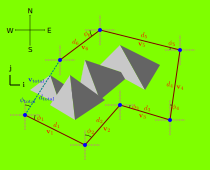
\includegraphics[width = 0.6\textwidth]{long_journey}
}
\end{tabular}

It is implicitly assumed that the positive x-direction is east, while the position y-direction is north. Using the above, the 6 displacement in component form are:
\begin{itemize}
\item \(\mathbf{v}_1 = \langle d_1\cos\phi_1 , -d_1\sin\phi_1 \rangle = \langle 3.000 , -1.000 \rangle\text{km}\)
\item \(\mathbf{v}_2 = \langle d_2\sin\phi_2 , d_2\cos\phi_2 \rangle = \langle 1.000 , 1.500 \rangle\text{km}\)
\item \(\mathbf{v}_3 = \langle d_3\cos\phi_3 , -d_3\sin\phi_3 \rangle = \langle 2.000 , -1.000 \rangle\text{km}\)
\item \(\mathbf{v}_4 = \langle d_4\sin\phi_4 , d_4\cos\phi_4 \rangle = \langle 0.5000 , 4.500 \rangle\text{km}\)
\item \(\mathbf{v}_5 = \langle -d_5\cos\phi_5 , d_5\sin\phi_5 \rangle = \langle -3.000 , 0.5000 \rangle\text{km}\)
\item \(\mathbf{v}_6 = \langle -d_6\cos\phi_6 , -d_6\sin\phi_6 \rangle = \langle -1.500 , -1.000 \rangle\text{km}\)
\end{itemize}
The total displacement is \(\mathbf{v}_\text{total} = \mathbf{v}_1 + \mathbf{v}_2 + \mathbf{v}_3 + \mathbf{v}_4 + \mathbf{v}_5 + \mathbf{v}_6 = \langle 2.000 , 3.500 \rangle\text{km}\). The final straight line distance \(d_\text{total}\) of the finishing point from the starting point is \(d_\text{total} = \|\mathbf{v}_\text{total}\| \approx 4.031\text{km}\). The direction of the final point from the starting point is \(\phi = \tan^{-1}(|2.000|/|3.500|) \approx 29.74^\circ\) east of north.



\end{document}











